% Phase-1 Project Proposal Report
% Password Manager -- DSA Project Based Learning with C++
% Compile with pdfLaTeX.

\documentclass[11pt,a4paper]{article}

\usepackage[a4paper,left=2.0cm,right=2.0cm,top=1.55cm,bottom=1.55cm]{geometry}
\usepackage[T1]{fontenc}
\usepackage{graphicx}
\usepackage{xcolor}
\usepackage{array}
\usepackage{tabularx}
\usepackage{ragged2e}
\usepackage{enumitem}
\usepackage{fancyhdr}
\usepackage{tikz}
\usepackage{setspace}
\usepackage{framed}
\usepackage{needspace}

% -------------------------------------------------
% COLOURS
% -------------------------------------------------
\definecolor{TitleBlue}{RGB}{61,103,154}

% -------------------------------------------------
% GENERAL SETTINGS
% -------------------------------------------------
\setlength{\parindent}{0pt}
\setlength{\parskip}{0pt}
\renewcommand{\arraystretch}{1.0}

\newcommand{\blueheading}[1]{%
    {\sffamily\color{TitleBlue}\fontsize{15}{18}\selectfont #1}%
}

\newcommand{\bluebigheading}[1]{%
    {\sffamily\bfseries\color{TitleBlue}\fontsize{16}{19}\selectfont #1}%
}

\newcommand{\instruction}[1]{%
    {\itshape\fontsize{10.5}{12.5}\selectfont #1}%
}

% Auto-sizing, page-breakable answer box: the border wraps tightly
% around whatever content is passed in (so text never overflows the
% frame), and -- unlike a plain \fbox{minipage}, which must jump
% entirely to the next page if it doesn't fit -- this box can split
% across a page break, so content fills each page instead of leaving
% large gaps of empty space.
\definecolor{AnswerBoxLine}{RGB}{0,0,0}
\setlength{\FrameSep}{2.5mm}
\setlength{\FrameRule}{0.4pt}
\newcommand{\answerbox}[2][]{%
    \vspace{2pt}
    \begin{framed}
    #2
    \end{framed}
}

% -------------------------------------------------
% HEADER / FOOTER
% -------------------------------------------------
\pagestyle{fancy}
\fancyhf{}
\renewcommand{\headrulewidth}{0pt}
\renewcommand{\footrulewidth}{0pt}

\fancyhead[L]{%
    \sffamily\bfseries\itshape\fontsize{10.5}{12}\selectfont
    DSA Project Based Learning with C++
}
\fancyhead[R]{%
    \sffamily\bfseries\fontsize{10.5}{12}\selectfont
    PROJECT PROPOSAL
}
\fancyfoot[R]{%
    \itshape\fontsize{10}{12}\selectfont
    Page \thepage
}
\setlength{\headheight}{14pt}
\setlength{\headsep}{23pt}
\setlength{\footskip}{24pt}

% -------------------------------------------------
% PAGE 1
% -------------------------------------------------
\begin{document}

\vspace*{4mm}

\bluebigheading{PROJECT AND TEAM INFORMATION}

\vspace{13mm}

\blueheading{Project Title}

\vspace{1mm}


\answerbox{Vaultify -- A Secure Command-Line Password Manager in C++}

\vspace{13mm}

\blueheading{Student / Team Information}

\vspace{2mm}

\noindent
\begin{tabularx}{\textwidth}{|>{\RaggedRight\arraybackslash}p{0.69\textwidth}|>{\RaggedRight\arraybackslash}X|}
\hline
\begin{minipage}[t]{\linewidth}
\vspace{1.5mm}
\textit{Team Id:}\\[-1mm]
\vspace{1.5mm}
\end{minipage}
&
\begin{minipage}[t]{\linewidth}
\vspace{1.5mm}
\textit{DSCPP-III-2026-T305}
\vspace{1.5mm}
\end{minipage}
\\
\hline
\begin{minipage}[t][3.9cm][t]{\linewidth}
\vspace{1.5mm}
\textbf{Team member 1 (Team Lead)}\\[-1mm]
\vspace{2mm}

% Photo placeholder -- replace with:
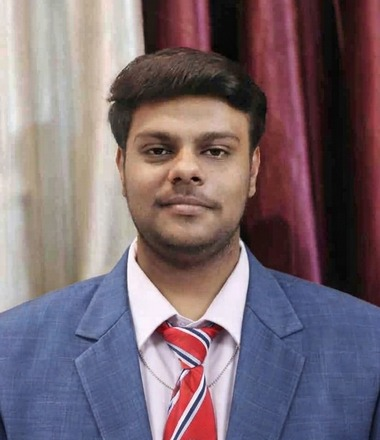
\includegraphics[width=1.9cm,height=2.2cm]{member1.jpg}
\end{minipage}
&
\begin{minipage}[t][3.9cm][t]{\linewidth}
\vspace{1.5mm}
\textit{Mishra, Ashraya}\\
\textit{Student ID: 2510010429}\\
\textit{Roll No.: 2027681}\\
\textit{Section : B}
\end{minipage}
\\
\hline
\begin{minipage}[t][3.9cm][t]{\linewidth}
\vspace{1.5mm}
\textbf{Team member 2}\\[-1mm]
\vspace{2mm}

% Photo placeholder -- replace with:
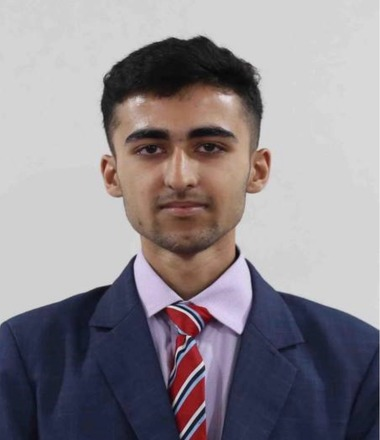
\includegraphics[width=1.9cm,height=2.2cm]{member2.jpg}
\end{minipage}
&
\begin{minipage}[t][3.9cm][t]{\linewidth}
\vspace{1.5mm}
\textit{Joshi, Udit}\\
\textit{Student ID: 2510370397}\\
\textit{Roll No.: 2028891}\\
\textit{Section : ML2}
\end{minipage}
\\
\hline
\begin{minipage}[t][3.9cm][t]{\linewidth}
\vspace{1.5mm}
\textbf{Team member 3}\\[-1mm]
\vspace{2mm}

% Photo placeholder -- replace with:
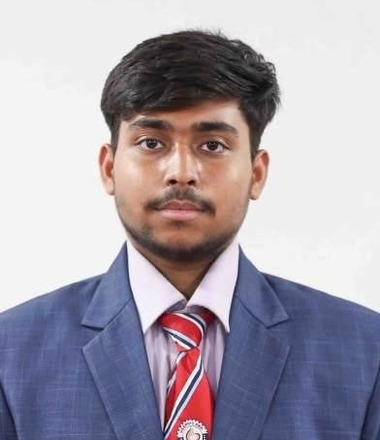
\includegraphics[width=1.9cm,height=2.2cm]{member3.jpg}
\end{minipage}
&
\begin{minipage}[t][3.9cm][t]{\linewidth}
\vspace{1.5mm}
\textit{Singh, Yuvraj}\\
\textit{Student ID: 2510010591}\\
\textit{Roll No.: 2028915}\\
\textit{Section: ML3}
\end{minipage}
\\
\hline
\end{tabularx}

\newpage

% -------------------------------------------------
% PAGE 2
% -------------------------------------------------

\bluebigheading{PROPOSAL DESCRIPTION}

\vspace{12mm}

\blueheading{Motivation}

\vspace{1mm}



\answerbox{The average internet user maintains accounts on dozens of websites and applications, yet human memory realistically allows for only a handful of passwords to be remembered reliably. As a result, most people either reuse the same password across multiple platforms or rely on weak, easily guessable passwords. This creates a serious security risk: when one website suffers a data breach, attackers routinely test the leaked credentials against other popular services (a technique known as credential stuffing), compromising accounts the user never intended to expose. Password managers address this problem directly by allowing a user to generate and store strong, unique passwords for every account while only needing to remember a single master password. This project aims to build a functional password manager from first principles, applying core data structures and object-oriented design concepts to solve a problem millions of people face daily.}

\vspace{12mm}

\blueheading{State of the Art / Current solution }

\vspace{1mm}


\answerbox{Password management today is dominated by commercial tools such as Bitwarden, LastPass, and 1Password, alongside browser-integrated managers built into Chrome, Firefox, and Safari. These tools are convenient and widely adopted, offering features like cross-device synchronization, browser autofill, and cloud backup. However, they are largely closed-source or proprietary systems -- users have limited visibility into how their credentials are actually stored, hashed, or encrypted internally, and must place complete trust in the vendor. Additionally, many advanced features are locked behind paid subscriptions, and browser-based managers tie credential storage to a single ecosystem. There is currently no lightweight, transparent, and freely inspectable alternative aimed at users or students who want to understand the underlying mechanics of secure credential storage rather than simply consuming a black-box product.}

\vspace{12mm}

\blueheading{Project Goals and Milestones}

\vspace{1mm}



\answerbox{The primary goal of this project is to design and implement a fully functional, secure command-line password manager in C++, applying core data structures (hash tables, stacks) and object-oriented programming principles (encapsulation, class design, file handling) taught in this course.

\textbf{Core Goals:}
\begin{itemize}[leftmargin=5mm, itemsep=0pt, topsep=2pt]
\item Implement a hash table-based vault for O(1) storage and retrieval of credentials by site name
\item Implement master password authentication using a hash-based verification scheme (master password is never stored in plain text)
\item Implement encryption/decryption of stored passwords using a symmetric cipher keyed on the master password
\item Implement persistent storage so the vault survives across sessions using file handling
\item Build a clean, menu-driven CLI supporting add, retrieve, update, delete, and list operations
\end{itemize}

\textbf{Stretch Goals:}
\begin{itemize}[leftmargin=5mm, itemsep=0pt, topsep=2pt]
\item Random strong password generator
\item Password strength checker for user-entered passwords
\item ``Recently accessed'' quick-view using a stack
\end{itemize}

\textbf{Milestones (aligned with course evaluation phases):}
\begin{itemize}[leftmargin=5mm, itemsep=0pt, topsep=2pt]
\item \textbf{TA1:} Finalize project scope, system design, and technology stack; complete initial setup of core class structure (Entry, Vault, Crypto modules)
\item \textbf{TA2:} Complete core functionality -- hash table vault, encryption/decryption, master password authentication, file persistence, and a working CLI; begin stretch goal implementation if time permits
\item \textbf{TA3:} Complete, polished, fully working project with all core features stable, stretch goals integrated where feasible, final report, and live demonstration
\end{itemize}}

\vspace{12mm}

\blueheading{Project Approach}

\vspace{1mm}





\answerbox{The project will be implemented in C++, using standard object-oriented design principles taught in this course. Development will follow a modular, bottom-up build order to ensure each component is independently testable before integration:

\begin{enumerate}[leftmargin=6mm, itemsep=0pt, topsep=2pt]
\item \textbf{Entry module} -- defines the class representing a single credential (site name, username, encrypted password) with proper encapsulation
\item \textbf{Vault module} -- implements the hash table that stores and retrieves \texttt{Entry} objects by site name, along with add/update/delete/list operations
\item \textbf{Crypto module} -- implements a symmetric encryption scheme to protect stored passwords, and a hash-based verification mechanism for master password authentication
\item \textbf{FileHandler module} -- handles serialization and deserialization of the vault to and from disk, ensuring persistence across sessions
\item \textbf{CLI module} -- ties all components together into a menu-driven command-line interface for the end user
\end{enumerate}

Development will be carried out using Visual Studio Code as the primary IDE, with GCC/g++ as the compiler. Git will be used for version control to track progress across the project phases, and the final report will be prepared using LaTeX for clean, professional formatting.}

\vspace{12mm}

\needspace{9cm}
\blueheading{System Architecture (High Level Diagram)}

\vspace{1mm}




\vspace{2pt}
\noindent
\fbox{%
    \begin{minipage}[t][7.6cm][t]{\dimexpr\textwidth-2\fboxsep-2\fboxrule\relax}
        \vspace{1mm}
        \centering
        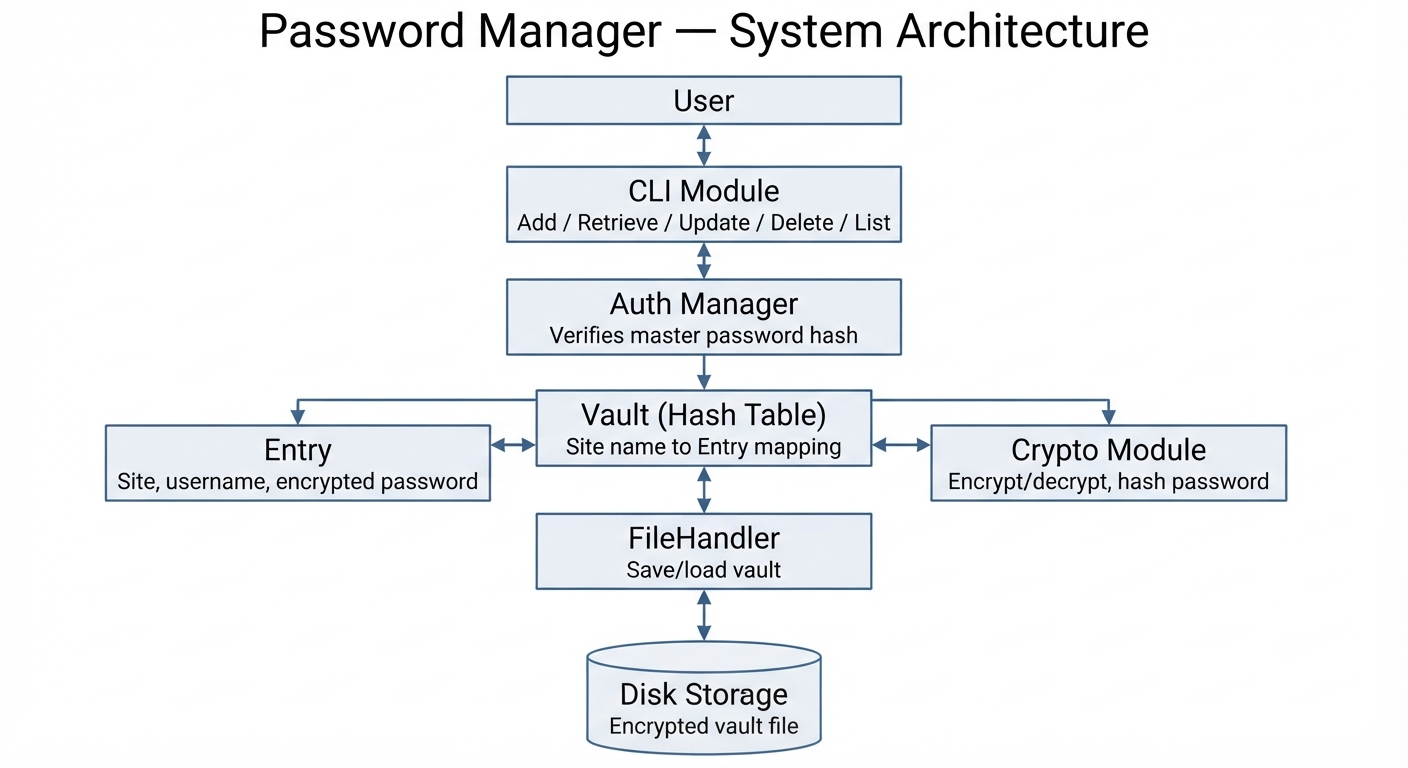
\includegraphics[width=0.95\linewidth,height=7.0cm,keepaspectratio]{architecture.png}
    \end{minipage}
}

\vspace{12mm}

\blueheading{Project Outcome / Deliverables}

\vspace{1mm}


\answerbox{By the completion of this project, the following deliverables will be produced:
\begin{itemize}[leftmargin=5mm, itemsep=0pt, topsep=2pt]
\item A fully functional, cross-platform C++ command-line password manager, compiled and tested on both Windows and Linux environments
\item Complete, well-documented source code implementing the Entry, Vault, Crypto, FileHandler, and CLI modules
\item A compiled executable ready for direct use
\item A final project report detailing the design, implementation, and technical outcomes of the project
\end{itemize}}

\vspace{12mm}

\blueheading{Assumptions}

\vspace{1mm}



\answerbox{This project assumes a single-user environment, where the tool is used by one individual on their own local machine, with no multi-user account support. It is assumed that the master password, once forgotten, cannot be recovered, as no password-recovery mechanism is implemented -- consistent with how real password managers protect vault contents. All credential data is stored locally on disk; no cloud synchronization or network transmission is involved. Finally, this project is developed for educational purposes to demonstrate core data structures and OOP concepts, and the encryption scheme used is not intended to meet production-grade security standards.}

\vspace{50mm}

\blueheading{References}

\vspace{1mm}



\answerbox{
\begin{enumerate}[leftmargin=5mm, itemsep=1pt, topsep=2pt]
\item Thareja, R. \textit{Data Structures Using C++}, Oxford University Press -- course textbook reference for hash tables, linked lists, and related data structure concepts.
\item cppreference.com -- official C++ language and standard library reference, consulted for syntax and standard practices.
\item GeeksforGeeks (geeksforgeeks.org) -- reference articles on hash table implementation, collision resolution, and file handling in C++.
\item OWASP Foundation (owasp.org) -- Password Storage Cheat Sheet, consulted for understanding real-world best practices around password hashing and storage (used as a conceptual benchmark, not directly implemented at production strength).
\item Course lecture notes and materials -- \textit{DSA Project Based Learning with C++}.
\end{enumerate}}

\end{document}
